\chapter{Planification du projet}

\section*{Introduction}
Ce chapitre commence par la spécification des besoins, en présentant les besoins fonctionnels et non fonctionnels. Ensuite, il aborde la gestion du projet avec Scrum, en présentant l'équipe Scrum, le backlog du produit et la planification de la release. Enfin, nous examinons l'environnement de développement, l'architecture et le patron de conception adaptés.

\section{Spécification des besoins}

Notre projet vise à développer une plateforme de marketplace d'API « Infinity API », permettant aux développeurs et aux entreprises d'intégrer et de consommer facilement des API de manière simplifiée. \\
Afin d'atteindre cet objectif, nous exposons les exigences fonctionnelles et non fonctionnelles de notre plateforme.

\subsection{Les besoins fonctionnels }
Les besoins fonctionnels de notre projet se résument comme suit :
\begin{itemize}
    \item  \textbf{Gestion des API}
          \begin{itemize}
              \item Ajout d’une API avec la documentation Swagger associée qui regroupe ainsi les endpoints, les descriptions des requêtes et des réponses, etc.
              \item Consultation, modification et suppression d'une API par un développeur.
          \end{itemize}
    \item \textbf{Gestion de la tarification des API}
          \begin{itemize}
              \item Création, modification et suppression de plans de tarification pour une API. Un plan de tarification est composé du nom du plan, du nombre de requêtes, de la durée d'utilisation de l'API et du prix.
              \item Consultation des plans de tarification disponibles pour une API.
          \end{itemize}
    \item \textbf{Catalogue d’API}
          \begin{itemize}
              \item Consultation de la liste des API par un utilisateur.
              \item Filtrage des APIs selon différents critères.
              \item Consultation des détails de chaque API.
          \end{itemize}
    \item \textbf{Gestion de la souscription à une API}
          \begin{itemize}
              \item Souscription à une API après avoir choisi le plan de tarification qui convient. Pour un plan de tarification payant, la souscription engendre une opération de paiement.
              \item Consultation de la liste des souscriptions.
              \item Mise à niveau de la souscription pour obtenir un quota de requêtes plus élevé et une durée de validité étendue.
              \item Annulation d’une souscription.
              \item Consultation de l'historique des paiements.
          \end{itemize}
    \item \textbf{Consommation et test des API}
          \begin{itemize}
              \item Consommation d’une API, qui consiste à utiliser les endpoints pour effectuer des requêtes et récupérer les données nécessaires.
              \item Test des API et leur consommation à travers la plateforme « Infinity API ».
          \end{itemize}
    \item \textbf{Gestion des "Payouts"} \\
          Un "Payout" est le terme technique utilisé pour désigner le versement effectué par la marketplace au fournisseur d'une API suite au paiement d'une souscription. Pour toute la suite du rapport, nous utilisons ce terme. \\
          La marketPlace doit permettre :
          \begin{itemize}
              \item Consultation du montant disponible sur le compte d’un développeur. Le montant correspond au total des paiements effectués lors de la souscription aux API fournies par le développeur après déduction des frais de la marketplace.          
              \item Consultation des transactions effectuées sur l’API fournie par un développeur.
              \item Demande d’un payout. 
              \item Gestion des demandes de payout par l'administrateur.
            \end{itemize}
    \item \textbf{Dashboard Administrateur}
          \begin{itemize}
              \item Consultation de la liste des développeurs inscrits sur la plateforme.
              \item Blocage et déblocage d’un compte développeur.
          \end{itemize}
    \item \textbf{Gestion des catégories} \\
    Ajout, modification, suppression et consultation de catégories qui définissent les types d'API.
    \item \textbf{Gestion des comptes utilisateur }
          \begin{itemize}
              \item Inscription d'un nouveau développeur.
              \item Consultation, modification d’un profil utilisateur.
              \item Suppression d'un profil développeur.
          \end{itemize}
    \item \textbf{Gestion des signalements de problèmes}
          \begin{itemize}
              \item Signalement d’un problème lié à une API.
              \item Consultation des signalements d'erreurs par l’administrateur et par le développeur qui a fourni l’API.
          \end{itemize}
\pagebreak

    \item \textbf{Gestion des feedbacks}
          \begin{itemize}
              \item Création, modification, et suppression d’un feedback(commentaire et note) relatif à une API.
              \item Consultation des feedbacks laissés par les développeurs.
          \end{itemize}
    \item \textbf{Suivi et statistiques }
           \begin{itemize}
                \item Suivi des statistiques sur l'utilisation de la plateforme.
                \item Suivi des statistiques de consommation des API.
                \item Suivi des statistiques de paiement des API.
                \item Suivi des statistiques de performance des API en terme de latence.
           \end{itemize}
    \item \textbf{Système de notifications  } \\
    La marketplace doit fournir des notifications en temps réel suite aux différentes opérations effectuées sur la plateforme. 
\end{itemize}
% Une deuxième sous section
\subsection{Les besoins non fonctionnels }
Les besoins non fonctionnels de notre projet se résument comme suit :
\begin{itemize}
    \item \textbf{Sécurité des données }
          \begin{itemize}
              \item Authentification des utilisateurs.
              \item Utilisation de mécanismes de sécurité pour protéger les données des utilisateurs.
              \item Sécurisation des payements.
          \end{itemize}
    \item \textbf{Ergonomie de l'interface }\\
          La navigation doit être intuitive et claire entre les différentes interfaces de l'application. \\
    
        La plateforme doit, également, répondre à certaines exigences techniques telles que: 
    \item \textbf{Documentation des API }\\
          La documentation doit utiliser Swagger.
    \item \textbf{Intégration de services de paiement en ligne }
          \begin{itemize}
            \item Le payement des souscriptions doit se faire avec Stripe.
            \item Les opérations de payout doivent s'effectuer via Paypal.
          \end{itemize}
\end{itemize}
\pagebreak


% Une deuxième section Pilotage du projet avec Scrum 
\section{Pilotage du projet avec Scrum }
Dans cette partie, nous allons aborder la présentation de l'équipe Scrum ainsi que le backlog du produit et pour finir, la planification de la release.
\subsection{Equipe et rôles  }
Avant de présenter le product backlog, il est important d'introduire l'équipe de travail :
\begin{itemize}
    \item \textbf{Le Product Owner }: M.Imed BEN MIMOUN : Vice Président.
    \item \textbf{Le Scrum Master }: M.Akram ANAYA : Chef projet de l’équipe de développement .
    \item \textbf{Les développeurs  }: Yassine LASSOUED et Ayoub SHILI.
\end{itemize}
\subsection{Le backlog du produit  }
Nous avons utilisé une échelle basée sur la suite de Fibonacci. Les valeurs attribuées sont les suivantes  : 1 pour "Très facile", 2 pour "Facile", 3 pour "Assez simple", 5 pour "Moyen", 8 pour "Assez compliqué", 13 pour "Compliqué" et 20 pour "Très compliqué". Dans le cas de notre marketPlace ,les utilisateurs sont :
\begin{itemize}
    \item \textbf{Visiteur }: c’est un internaute qui n'a pas encore été authentifié.
    \item \textbf{Développeur  }: qui est inscrit sur notre plateforme, il peut jouer le rôle de fournisseur ou de consommateur d’API
    \item \textbf{Administrateur }: qui gère la plateforme.
\end{itemize}



% Define colors



\definecolor{lightgray}{gray}{0.9}

\captionsetup[table]{justification=centering}




\begin{landscape}
\begin{longtable}[c]{
    |p{.15\textwidth}
    |p{.05\textwidth}
    |p{.75\textwidth}
    |p{.10\textwidth}
    |p{.05\textwidth}
    |p{.10\textwidth}|
    }
    \caption{Le backlog du produit}
    \label{tab} \\
    \hline
    \textbf{Thème} &  \textbf{US ID} & \textbf{User Story} & \textbf{Valeur Business} & \textbf{Effort} & \textbf{Priorité} \\
    \hline
    \endfirsthead   
    \hline
    \textbf{Thème} &  \textbf{US ID} & \textbf{User Story} & \textbf{Valeur Business} & \textbf{Effort} & \textbf{Priorité} \\
    \hline
    \endhead
    \hline
    \endfoot
    \hline
    \endlastfoot
Création du compte Utilisateur & 1 & En tant que visiteur, je souhaite pouvoir m'inscrire pour créer un compte. & Haute & 5 & Haute \\
\hline
Authentification & 2 & En tant que développeur ou administrateur, je souhaite pouvoir m'authentifier pour accéder à mon compte. & Haute & 13 & Haute \\
\hline
 & 3 & En tant qu'administrateur, je veux créer une nouvelle catégorie en spécifiant son nom, sa description et d'autres informations pertinentes. & Haute & 3 & Haute \\
\cline{2-2} \cline{3-6}

Gestion des catégories & 4 & En tant qu'administrateur, je veux modifier les détails d'une catégorie existante. & Haute & 3 & Haute \\
\cline{2-2} \cline{3-6}

 & 5 & En tant qu'administrateur, je veux supprimer une catégorie. & Haute & 2 & Haute \\
\cline{2-2} \cline{3-6}

 & 6 & En tant qu'administrateur, je veux consulter la liste des catégories existantes sur la plateforme. & Haute & 3 & Haute \\
\hline
 & 7 & En tant que développeur, je veux pouvoir ajouter une nouvelle API pour fournir une API aux autres utilisateurs. & Haute & 20 & Haute \\
\cline{2-2} \cline{3-6}
Gestion des APIs & 8 & En tant que développeur, je veux consulter la liste de mes APIs pour visualiser rapidement toutes les APIs que j'ai créées. & Haute & 5 & Haute \\
\cline{2-2} \cline{3-6}
 & 9 & En tant que développeur, je veux pouvoir modifier les informations de mon API pour mettre à jour les informations. & Haute & 5 & Haute \\
\cline{2-2} \cline{3-6}
 & 10 & En tant que développeur, je veux pouvoir supprimer mon API car elle n'existe plus ou contient beaucoup de signalements d'erreurs. & Haute & 2 & Haute \\
\hline

Consultation, filtrage et recherche sur les APIs & 11 & En tant que visiteur, développeur ou administrateur, je veux pouvoir consulter la liste des APIs pour pouvoir chercher l’API qui répond à mes besoins. & Haute & 5 & Haute \\
\cline{2-2} \cline{3-6}

 & 12 & En tant que visiteur, développeur ou administrateur, je veux pouvoir consulter les détails d'une API pour découvrir ses fonctionnalités. & Haute & 8 & Haute \\
\cline{2-2} \cline{3-6}

 & 13 & En tant que visiteur, développeur ou administrateur, je veux pouvoir rechercher une API par son nom pour la trouver rapidement et facilement. & Haute & 2 & Haute \\
\cline{2-2} \cline{3-6}

 & 14 & En tant que visiteur, développeur ou administrateur, je veux pouvoir faire un filtrage avancé sur les APIs pour trouver celles qui correspondent le mieux à mes besoins. & Haute & 5 & Haute \\
\hline
 & 15 & En tant que développeur ou administrateur, je veux pouvoir consulter mon profil pour vérifier mes informations personnelles. & Haute & 3 & Haute \\
\cline{2-2} \cline{3-6}
Gestion du compte Utilisateur & 16 & En tant que développeur ou administrateur, je veux pouvoir modifier mon profil pour mettre à jour mes informations. & Haute & 5 & Haute \\
\cline{2-2} \cline{3-6}
 & 17 & En tant que développeur, je veux pouvoir supprimer mon compte pour me désinscrire de la plateforme. & Haute & 2 & Haute \\
\hline

 & 18 & En tant que développeur, je veux pouvoir créer des plans de tarification pour mon API pour proposer différents niveaux d'accès à mon API et générer des revenus. & Moyenne & 8 & Haute \\
\cline{2-2} \cline{3-6}

 & 19 & En tant que développeur, je veux pouvoir consulter les plans de tarification pour suivre les options disponibles pour mes APIs. & Moyenne & 3 & Haute \\
\cline{2-2} \cline{3-6}

Gestion de la tarification  & 20 & En tant que développeur, je veux pouvoir modifier des plans de tarification pour mon API pour pouvoir mettre à jour les prix et les limites d'utilisation. & Moyenne & 5 & Haute \\
\cline{2-2} \cline{3-6}

 & 21 & En tant que développeur, je veux pouvoir supprimer un plan de tarification pour mon API si la tarification n'est plus nécessaire. & Moyenne & 2 & Haute \\
\cline{2-2} \cline{3-6}

 & 22 & En tant qu'utilisateur, je veux pouvoir consulter les plans de tarification pour une API afin de choisir celui qui correspond le mieux à mes besoins et à mon budget. & Moyenne & 3 & Haute \\
\hline
 & 23 & En tant que développeur, je veux pouvoir souscrire à une API pour accéder aux fonctionnalités qu'elle propose. & Moyenne & 20 & Haute \\
\cline{2-2} \cline{3-6}
Souscription & 24 & En tant que développeur, je veux pouvoir consulter la liste de mes souscriptions pour suivre mes souscriptions. & Moyenne & 2 & Haute \\
\cline{2-2} \cline{3-6}
 & 25 & En tant que développeur, je veux pouvoir effectuer une mise à niveau de ma souscription d'API. & Moyenne & 8 & Haute \\
\cline{2-2} \cline{3-6}
 & 26 & En tant que développeur, je veux pouvoir annuler une souscription. & Moyenne & 3 & Haute \\
\hline

Consommation et test d'une API & 27 & En tant que développeur ou administrateur, je veux pouvoir consommer une API et l'intégrer dans mon projet afin d'utiliser ses fonctionnalités. & Moyenne & 13 & Haute \\
\cline{2-2} \cline{3-6}

 & 28 & En tant que développeur ou administrateur, je veux pouvoir tester l'API sur la plateforme pour savoir si elle fonctionne correctement et qu'elle répond aux besoins de mon application. & Moyenne & 13 & Haute \\
\hline
 & 29 & En tant qu'administrateur, je veux pouvoir consulter la liste des développeurs et suivre leurs activités. & Moyenne & 3 & Moyenne \\
\cline{2-2} \cline{3-6}
Dashboard Administrateur & 30 & En tant qu'administrateur, je veux pouvoir rechercher un utilisateur. & Moyenne & 2 & Moyenne \\
\cline{2-2} \cline{3-6}
 & 31 & En tant qu'administrateur, je veux pouvoir consulter les détails d'un développeur pour comprendre son activité et ses interactions avec la plateforme. & Moyenne & 8 & Moyenne \\
\cline{2-2} \cline{3-6}
 & 32 & En tant qu'administrateur, je veux pouvoir bloquer/débloquer un compte développeur pour contrôler tout comportement abusif ou non autorisé. & Moyenne & 3 & Moyenne \\
\hline

& 33 & En tant que développeur, je veux pouvoir consulter le montant disponible sur mon compte afin de suivre mes revenus générés par la vente d'API sur la plateforme. & Moyenne & 3 & Moyenne \\
\cline{2-2} \cline{3-6}

  & 34 & En tant que développeur, je souhaite pouvoir consulter l'historique des demandes de payout effectuées via mon API afin de retracer l'origine de mes revenus.& Moyenne & 3 & Moyenne \\
\cline{2-2} \cline{3-6}

 & 35 & En tant que développeur, je souhaite pouvoir lier mon compte PayPal à mon compte afin de pouvoir réaliser des demandes de paiement. & Moyenne & 5 & Moyenne \\
 \cline{2-2} \cline{3-6}
 
 Gestion des payouts & 36 &  En tant que développeur, je souhaite avoir la possibilité de supprimer la liaison entre mon compte PayPal et mon compte sur la plateforme & Moyenne & 2 & Moyenne \\
  \cline{2-2} \cline{3-6}
  
   & 37 &    En tant que développeur, je souhaite avoir la possibilité de changer le compte PayPal associé à mon compte sur la plateforme & Moyenne & 3 & Moyenne \\
  \cline{2-2} \cline{3-6}

 & 38 & En tant que développeur, je veux pouvoir effectuer une demande de payout du solde disponible sur le compte. & Moyenne & 3 & Moyenne \\
\cline{2-2} \cline{3-6}

 & 39 & En tant qu'administrateur, je veux pouvoir gérer les demandes de payout en les acceptant ou en les refusant. & Moyenne & 3 & Moyenne \\
\hline
 & 40 & En tant que développeur ou administrateur, je veux pouvoir suivre les statistiques de performance d'une API pour connaître sa qualité de service. & Faible & 13 & Moyenne \\
\cline{2-2} \cline{3-6}
Dashboards de Statistiques & 41 & En tant que développeur, je veux pouvoir suivre les statistiques d'utilisation de mon API (nombre de requêtes, nombre de développeurs, etc.) pour suivre l'utilisation de mon API. & Faible & 13 & Moyenne \\
\cline{2-2} \cline{3-6}
 & 42 & En tant qu'administrateur, je veux pouvoir suivre les statistiques des paiements sur la plateforme pour surveiller les revenus de la plateforme. & Faible & 13 & Moyenne \\
\hline

 & 43 & En tant que développeur, je veux pouvoir signaler un problème pour obtenir une assistance ou signaler des problèmes de fonctionnement. & Faible & 5 & Moyenne \\
\cline{2-2} \cline{3-6}

Gestion des signalements & 44 & En tant que développeur, je veux pouvoir consulter mes signalements d'erreurs. & Faible & 3 & Moyenne \\
\cline{2-2} \cline{3-6}

 & 45 & En tant qu'administrateur, je veux pouvoir consulter les signalements d'erreur pour suivre les problèmes identifiés par les développeurs. & Faible & 3 & Faible \\
\hline
 & 46 & En tant que développeur, je veux pouvoir ajouter un feedback à une API pour partager mon avis sur l'API. & Faible & 3 & Faible \\
\cline{2-2} \cline{3-6}
 & 47 & En tant que développeur, je veux pouvoir consulter les feedbacks laissés par les développeurs d'une API afin de connaître leur opinion sur celle-ci. & Faible & 2 & Faible \\
\cline{2-2} \cline{3-6}
Gérer les feedbacks & 48 & En tant que développeur, je veux pouvoir modifier mon feedback si je souhaite le rectifier. & Faible & 2 & Faible \\
\cline{2-2} \cline{3-6}
 & 49 & En tant que développeur, je veux pouvoir supprimer mon feedback si je souhaite le retirer de la plateforme. & Faible & 2 & Faible \\
\cline{2-2} \cline{3-6}
 & 50 & En tant que administrateur, je veux pouvoir supprimer mon feedback si je souhaite le retirer de la plateforme. & Faible & 2 & Faible \\
\hline

Système de notification & 51 & En tant que développeur ou administrateur, je veux pouvoir consulter les notifications. & Faible & 8 & Faible \\
\hline
\end{longtable}
\end{landscape}




\subsection{Planification de la release }
La planification de la release est une pratique agile consistant à diviser le travail en itérations courtes. Nous avons découpé notre release en 3 sprints de 4 semaines, comme l’illustre le tableau suivant.

\begin{longtable}[c]{
    |p{.15\textwidth}
    |p{.25\textwidth}
    |p{.25\textwidth}
    |p{.25\textwidth}|
    }
    \caption{Plannification de la release}
    \label{tab:sprintplanning}                                                                                                                                                                                                                                                                                                                                                                                                                         \\
    \hline
    \textbf{}                                                                                                                                                                                                                                                            & \textbf{Sprint 1}            & \textbf{Sprint 2}            & \textbf{Sprint 3}                                                                                             \\
    \hline
    \endfirsthead
    \multicolumn{4}{c}%
    {{\bfseries \tablename\ \thetable{} -- suite de la page précédente}}                                                                                                                                                                                                                                                                                                                                                                               \\
    \hline
    \textbf{}                                                                                                                                                                                                                                                            & \textbf{Sprint 1}            & \textbf{Sprint 2}            & \textbf{Sprint 3}                                                                                             \\
    \hline
    \endhead
    \endfoot
    \hline
    \endlastfoot

    \textbf{Date début et fin}        & Du 04-03-2024 au 30-03-2024 & Du 01-04-2024 au 27-04-2024 & Du 29-04-2024 au 25-05-2024                                                                                  \\
    \hline
    \textbf{Objectif}                                                                                                                                                                                                                                                    &
    L'objectif du sprint 1 est de fournir aux utilisateurs la possibilité de créer leur compte utilisateur, ainsi que de créer une API et de la rendre disponible sur la marketplace et de gérer leur profil.                                                            &
    L'objectif du sprint 2 est de permettre aux utilisateurs d'intégrer la tarification dans leur API, de gérer leurs souscriptions, de consommer les APIs disponibles dans le catalogue et de développer un tableau de bord administrateur pour gérer les utilisateurs. &
    L'objectif du sprint 3 est de développer un tableau de bord permettant aux utilisateurs d'analyser l'utilisation de leurs APIs via des statistiques et de gérer leurs transactions. Il vise également à permettre aux administrateurs de suivre les statistiques des APIs et des paiements. De plus, il inclut la mise en place d'un système de notifications pour la gestion des signalements et des messages ainsi que la gestion des feedbacks. \\
    \hline
    \textbf{Les User Stories}  & 1 jusqu’à 17   & 18 jusqu’à 32  & 33 jusqu’à  51                                                                                                 \\
    \hline
    \textbf{Estimation}   & 91    & 94       & 93                                                                                                          \\
    \hline
\end{longtable}

\section{Environnement de travail}
Cette partie présente spécifiquement l'environnement matériel et logiciel utilisés pour mettre en œuvre notre application.
\subsection{Environnement matériel }
Les matériels utilisés pour notre projet se résument comme suit :
\begin{longtable}[c]{
    |p{.35\textwidth}
    |p{.3\textwidth}
    |p{.25\textwidth}|
    }
    \caption{Spécifications des Ordinateurs}
    \label{tab:computerspecs}                                                                                                   \\
    \hline
    \textbf{Nom de l'ordinateur}    & \textbf{Yassine-MSI}                          & \textbf{Asus-PC}                          \\
    \hline
    \endfirsthead
    \multicolumn{3}{c}%
    {{\bfseries \tablename\ \thetable{} -- suite de la page précédente}}                                                        \\
    \hline
    \textbf{Nom de l'ordinateur}    & \textbf{Yassine-MSI}                          & \textbf{Asus-PC}                          \\
    \hline
    \endhead
    \hline \multicolumn{3}{|r|}{{\bfseries Suite à la page suivante}}                                                           \\ \hline
    \endfoot
    \hline
    \endlastfoot

    \textbf{Processeur}             & 10th Gen Intel® Core™ i7-1015G4 @ 3.00GHz × 4 & 11th Gen Intel® Core™ i5-11400H @ 2.70GHz \\
    \hline
    \textbf{RAM}                    & 24 Go                                         & 16 Go                                     \\
    \hline
    \textbf{Disque Dur}             & 1 To HDD + 512 Go SSD                         & 1 To SSD                                  \\
    \hline
    \textbf{Système d'exploitation} & Windows 11                                    & Windows 11                                \\
    \hline
\end{longtable}
\subsection{Environnement logiciel  }
Les logiciels, Bibliothèques et Frameworks pour notre projet se résument comme suit :


\begin{longtable}[c]{
    |p{.15\textwidth}
    |p{.85\textwidth}|
    }
    \caption{Description des Logiciels, Bibliothèques et Frameworks}
    \label{tab:softwaredesc}                                                                                                                                                                                                                                                                                                                                                    \\
    \hline
    \textbf{Logiciels, Bibliothèques et Frameworks}                                             & \textbf{Description}                                                                                                                                                                                                                                                                                            \\
    \hline
    \endfirsthead
    \hline
    \endhead
    \hline
    \endfoot
    \hline
    \endlastfoot

    \vspace{0.5 mm}
    
\includegraphics[width=0.1\textwidth]{angular_logo.png}   &\textbf{ Angular 17}   : est un Framework côté client (front end) à code source ouvert basé sur TypeScript dirigé par l’équipe du projet Angular de Google qui permet de construire des applications web dynamiques.\cite[]{angular}                                                                                                   \\
    \hline
    \vspace{0.5 mm}
    
\includegraphics[width=0.1\textwidth]{tailwind_logo.png}  & \textbf{ Tailwind UI} : est une collection de composants d'interface utilisateur entièrement réactifs. Il propose des centaines d'exemples prêts à l'emploi.   \cite[]{tailwind}                                                                                                                                                  \\
    \hline
    \vspace{0.5 mm}
    
\includegraphics[width=0.1\textwidth]{Angular-material.png}  & \textbf{ Angular material } :     Il permet aux développeurs de créer des applications web professionnelles et modernes en utilisant des composants tels que des boutons, des barres de navigation, des formulaires, des boîtes de dialogue, ainsi que différentes autres options. \cite[]{angularMaterial}   \\
    \hline
    \vspace{0.5 mm}
    
\includegraphics[width=0.1\textwidth]{swagger_logo.png}   & \textbf{Swagger UI }:permet de visualiser et d'interagir avec les ressources de l'API sans qu'aucune logique de mise en œuvre ne soit en place. Il est automatiquement généré à partir de la spécification OpenAPI avec la documentation visuelle facilitant la mise en œuvre du back-end et la consommation côté client. \cite[]{OutilSwagger}\\
    \hline
    \vspace{0.5 mm}
    
\includegraphics[width=0.1\textwidth]{nodejs_logo.png}    & \textbf{Node JS 20} : est un environnement permettant d'exécuter du code JavaScript hors d'un navigateur. Il repose sur le moteur JavaScript V8 développé par Google pour ses navigateurs Chrome et Chromium.   \cite[]{nodeJS}                                                                                                         \\
    \hline
    \vspace{0.5 mm}
    
\includegraphics[width=0.1\textwidth]{expressjs_logo.png} & \textbf{Express JS }: est une infrastructure d'applications Web Node.js minimaliste et flexible qui fournit un ensemble de fonctionnalités robuste pour les applications Web et mobiles.  \cite[]{ExpressJS}                                                                                                                               \\
    \hline
    \vspace{0.5 mm}
    
\includegraphics[width=0.1\textwidth]{mongodb_logo.png}   & \textbf{MongoDB }: est un système de gestion de base de données orienté documents (NoSQL), répartissable sur un nombre quelconque d'ordinateurs et ne nécessitant pas de schéma prédéfini des données. Il est écrit en C++.   \cite[]{Mongodb}                                                                                           \\
    \hline
    \vspace{0.5 mm}
    
\includegraphics[width=0.1\textwidth]{vscode_logo.png}    & \textbf{ Visual Studio Code }: est un éditeur de code cross-platforme, code source ouvert et gratuit, supportant une dizaine de langages de développement.  \cite[]{vscode}                                                                                                                                                              \\
    \hline
    \vspace{0.5 mm}
    
\includegraphics[width=0.1\textwidth]{postman_logo.png}   & \textbf{ Postman }: permet de construire et d’exécuter des requêtes HTTP, de les stocker dans un historique afin de pouvoir les rejouer, mais surtout de les organiser en collections.     \cite[]{postman}                                                                                                                             \\
    \hline
    \vspace{0.5 mm}
    
\includegraphics[width=0.1\textwidth]{Figma-logo.jpg}   & \textbf{Figma} :   permet aux utilisateurs de créer, partager et tester différents designs pour des sites Web, des applications mobiles et d'autres produits. \cite[]{Figma}      \\
    \hline
    \vspace{0.5 mm}
    
\includegraphics[width=0.1\textwidth]{github_logo.png}    & \textbf{ GitHub}: est un site web et un service de cloud qui aide les développeurs à stocker et à gérer leur code, ainsi qu’à suivre et contrôler les modifications qui lui sont apportées. \cite[]{gitHub}                                                                                                                               \\
    \hline
    \vspace{0.5 mm}
    
\includegraphics[width=0.1\textwidth]{staruml_logo.png}   & \textbf{StarUML} : Il s'agit d'un outil pour créer des diagrammes UML (Unified Modeling Language), qui permet de créer par exemple des diagrammes de classes, des diagrammes de cas d'utilisation, des diagrammes de séquence et d'autres types de diagrammes.                                                           \\
    \hline

\end{longtable}


\section{Architecture et patron de conception }
\subsection{Architecture adoptée }
L'architecture MEAN est une pile technologique populaire pour le développement d'applications web. Elle est composée de quatre composants principaux : MongoDB, Express, Angular et Node.js. Chaque composant joue un rôle spécifique dans le développement d'une application web. MongoDB est utilisé pour stocker les données de l'application, Express est utilisé pour créer l'API web, Angular est utilisé pour créer l'interface utilisateur et Node.js est utilisé pour exécuter le code JavaScript côté serveur.La figure suivante illustre l'architecture MEAN
\begin{figure}[H]
    \centering
    \frame{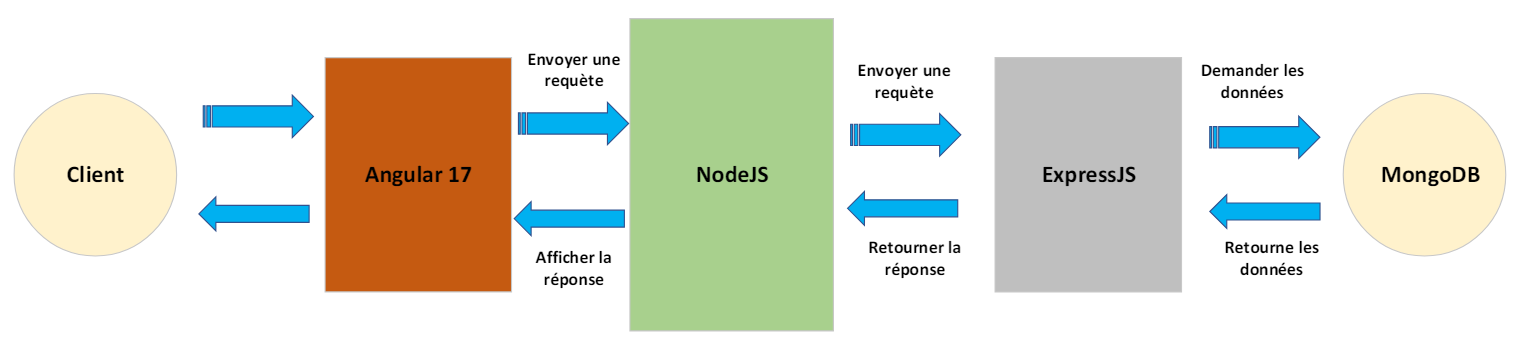
\includegraphics[width=0.9\columnwidth,]{img/Architecture_MEAN.png}}
    \caption{Architecture MEAN }
    \label{fig:logo_tt}
\end{figure}
\subsection{  Patron de conception adopté }
Le MVC est un motif de conception (design pattern) qui sépare une application en trois composants logiques principaux : modèle, vue et contrôleur. Il propose une solution générale au problème de la structuration d’une application comme le montre la figure 2.2 \\
Dans notre projet, le choix de ce modèle est exigé par le framework front-end   Angular, et le framework back-end Node js \\
Le fonctionnement du patron est illustré à travers la figure suivante : 
\begin{figure}[H]
    \centering
    \frame{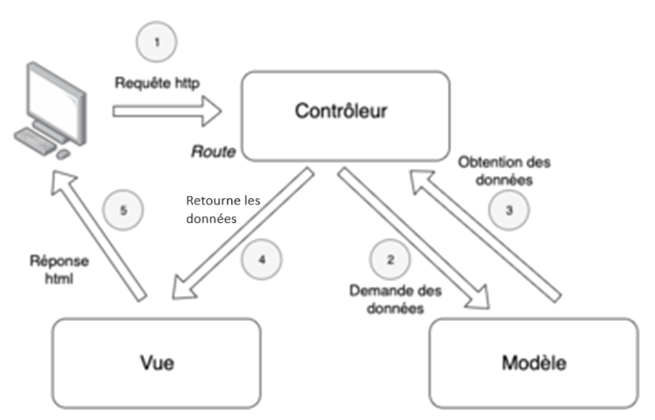
\includegraphics[width=0.8\columnwidth]{img/Architecture_MVC.png}}
    \caption{Architecture MVC \cite[]{MVC} }
    \label{fig:logo_tt}
\end{figure}
\section*{Conclusion}
Dans ce chapitre, nous avons préparé notre plan de travail. Nous avons présenté les besoins fonctionnels et non fonctionnels, les tâches des acteurs, le product backlog ainsi que la planification de la release, l'environnement de travail, l'architecture et le patron de conception à adopter. Dans le chapitre suivant, nous allons présenter le sprint 1